\documentclass[12pt]{article}

\usepackage{fancyhdr,hyperref,setspace,booktabs,amsmath,multirow}
\usepackage[pdftex]{graphicx}
\usepackage[margin=1in,includehead,headheight=15pt]{geometry}

\usepackage[backend=bibtex,style=numeric,maxnames=99,isbn=false,url=true]{biblatex}
\renewbibmacro{in:}{}
\addbibresource{paper.bib}

\pagestyle{fancy}
\lhead{Miriam Gershenson, Ben Kraft, and Ryan Lau}
\rhead{6.S897/17.S952 Final Paper}

\begin{document}

  \begin{center}
    \LARGE Comparing Metrics of Gerrymandering
    \vspace{-0.5em}
  \end{center}
  \nocite{*}
  \doublespacing{}

  \section{Introduction}

  In any legislature where each representative is elected by a separate district, someone has to draw the districts. Deciding the lines is a subjective task which can have major implications for the balance of power in the resulting legislature, so naturally it is sometimes done with some goal other than fairness in mind. This practice is so common that a word for it, ``gerrymandering'', was coined after Massachusetts governor Elbridge Gerry drew a district that looked like a salamander and is still in common use.

There are a few possible motivations for gerrymandering. One is straightforward partisan advantage. When districts are drawn by a politically biased body, often a legislature with a strong majority for one party, it will often draw the districts to suit its bias. Another is incumbent protection. In some cases, neither party in a legislature has enough of a majority to draw districts to cement its advantage, but both can agree to create better chances of reelection for everyone involved. Finally, sometimes districts are intentionally created with a very large racial minority population. This can be done either with the intent of creating more minority representation in the legislature, or as part of a standard partisan gerrymander.

There are legal limits on the creation of biased districts, but there is no accepted test of whether or not gerrymandering has occurred. Courts can look at a plan and decide whether the redistricting plan appears to be biased, often based on the presence of districts with strange shapes. However, laws against gerrymandering could have a stronger effect if there were an accepted objective way of measuring it.

In this paper, we compare some of the metrics of gerrymandering that have been proposed. They include metrics based on the shape of districts, metrics based on population in the district and the surrounding area, and a recently proposed metric that measures the resulting bias.

  \section{Background}\label{s:background}

  \subsection{Measuring Compactness}

  When people think of measuring gerrymandering, the first kind of metric that comes to mind is generally one that tries to measure the compactness of a district.  In fact, there are a number of ways of measuring compactness; some are better than others, but many measure different types of compactness.  There are three major types: those that measure the dispersion of the district from its center, those that measure some form of boundary complexity, and those that are based on population and population density.
% TODO: maybe this wants a figure to show some of the metrics visually? I would make one but my laptop crashes when I try to use qgis. At least convex hull probably wants this, maybe also circumscribing/inscribed circle although those matter less since we never computed them.

  The very simplest metrics for compactness simply measure the length and width of the district as compared to that of a circle or rectangle of the same area.  There are several variations on this method, but they are all fairly crude.  Other metrics compare the area of the district to the area of the smallest circumscribing circle, or the largest inscribed circle, or to the convex hull of the district -- the smallest convex shape containing the entire district.  Niemi~et~al.~\cite{niemi} list a number of variations on these metrics.  An alternate method of computing dispersion is by computing the moment of inertia of the area of the district.  The concept is borrowed from physics, and is defined as
  \[I = \iint \left((x-x_0)^2 + (y-y_0)^2\right) dx\, dy \]
  where $(x_0, y_0)$ is the center of mass of the district (weighted by area).  More dispersed districts have higher moments of inertia, because the average square distance of a point in the district to the center is larger.  In order to ensure that the metric does not depend on the size of the state, and to make it range from 0 to 1 with 0 being the least compact, we in fact use the measure $A/\sqrt{2\pi I}$.  This metric seems to have been first proposed by Kaiser.~\cite{kaiser}

  These dispersion measures capture well the extent to which a district is spread out more than necessary -- barbell- and snake-shaped districts score poorly.  However, districts with very complex boundaries aiming to pick up exactly the voters who will advantage one party can still be fairly concentrated close to their centers.  These districts are better detected by measures of boundary complexity.  The usual way to measure this is the perimeter.  In order to account for the varying sizes of districts and states, one can compare the perimeter to that of a circle of the same area, by using the metric $4\pi A/P^2$; several variations are given by Horn.~\cite{horn}  There are some other metrics for boundary complexity which attempt to account for the complexity of existing political boundaries, such as one given by Schwartzberg~\cite{schwartzberg} that measures distances between intersections of political divisions.

  Lastly, since ultimately it is not the geography that matters, but the people that live in it, we can modify some of these metrics to take into account population.  Those that compare the area of the district to that of the smallest circumscribing circle or that of the convex hull of the district may simply compare population instead of area, as proposed by Hofeller and Grofman.~\cite{hofeller}.  Alternately, instead of computing the area-weighted moment of inertia, one can compute the population-weighted moment of inertia, which is defined as
  \[I_P = \iint \left((x-x_0)^2 + (y-y_0)^2\right) \rho\, dx\, dy \]
  where $\rho$ is the population density and $(x_0, y_0$ is the center of mass of the district, now weighted by population.  In practice, since we do not know the location of each individual in the district, we may simply assume that each person lives at the center of the census tabulation block in which they were counted.  Then the formula becomes
  \[I_P = \sum_{b} \left((x_b-x_0)^2 + (y_b-y_0)^2\right) P_b\]
  where the sum is taken over census tabulation blocks $b$, with $(x_b, y_b)$ the center of mass (weighted by area) of the census block, and $P_b$ its population.  In order to make the metric less dependent on population, we can use the metric $AP_d/(2\pi I_P)$; this does not necessarily normalize the metric to be between 0 and 1, but at least makes it independent of the total area and total population.  Using moment of population to measure district compactness was first proposed by Weaver.~\cite{weaver}

  \begin{figure}
    \begin{center}
      \parbox{0.49\textwidth}{\centering 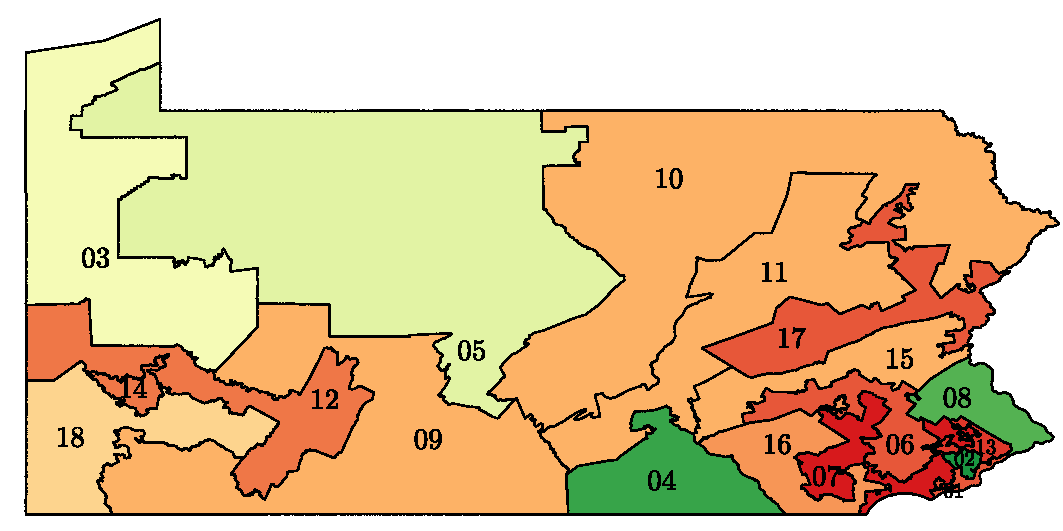
\includegraphics[width=0.48\textwidth]{map-area_per.pdf} \\ Area vs. Perimeter}
      \parbox{0.49\textwidth}{\centering 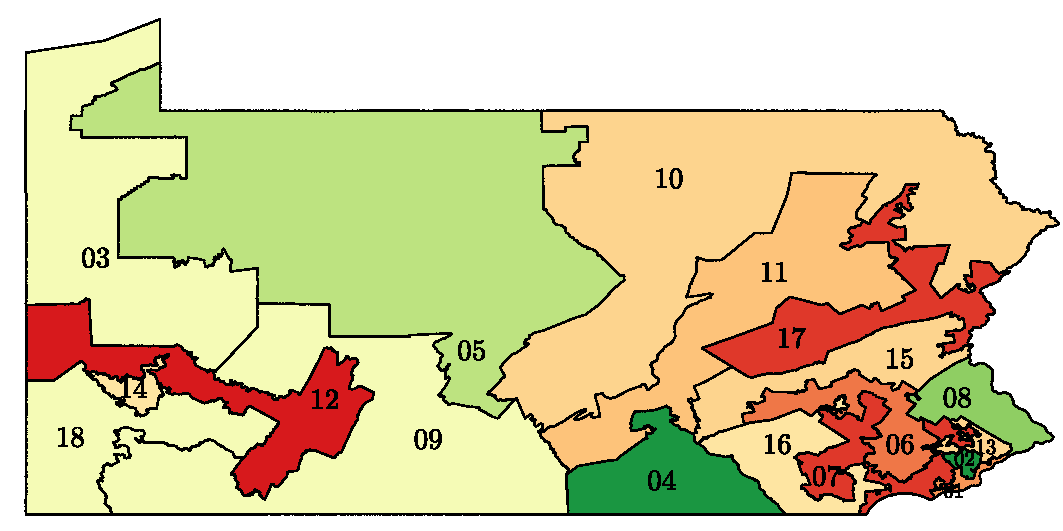
\includegraphics[width=0.48\textwidth]{map-convex_hull.pdf} \\ Convex Hull Area}
      \parbox{0.49\textwidth}{\centering 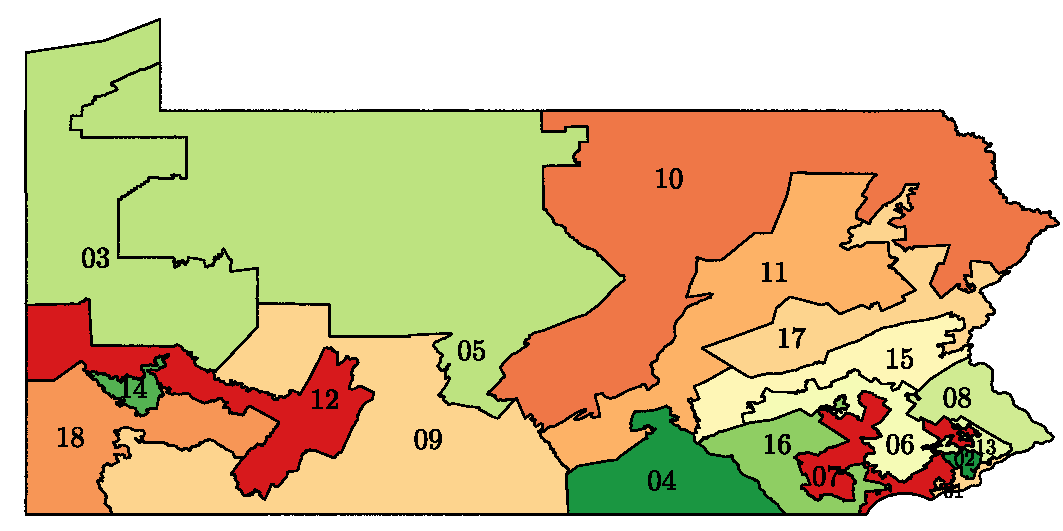
\includegraphics[width=0.48\textwidth]{map-convex_hull_pop.pdf} \\ Convex Hull Population}
      \parbox{0.49\textwidth}{\centering 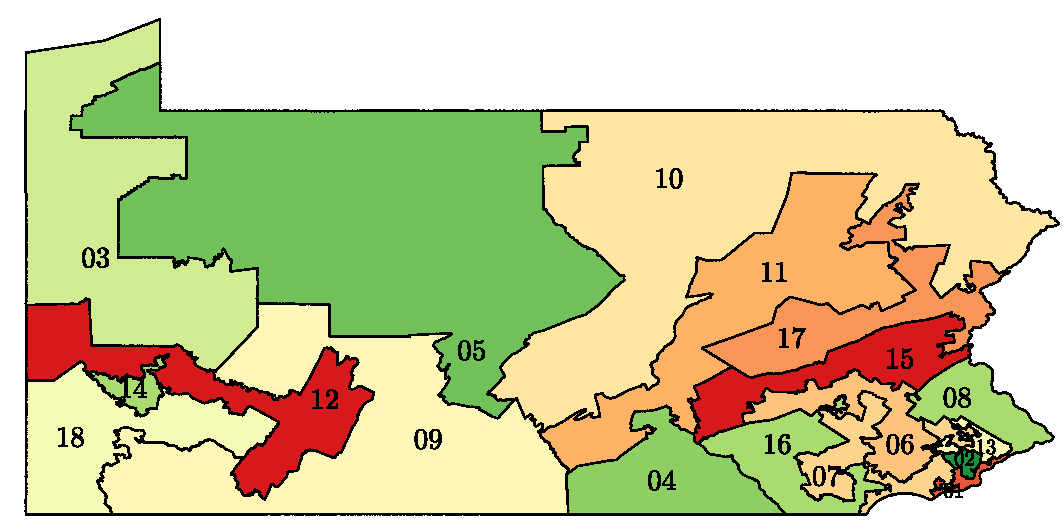
\includegraphics[width=0.48\textwidth]{map-moment_area.pdf} \\ Moment of Area}
      \parbox{0.49\textwidth}{\centering 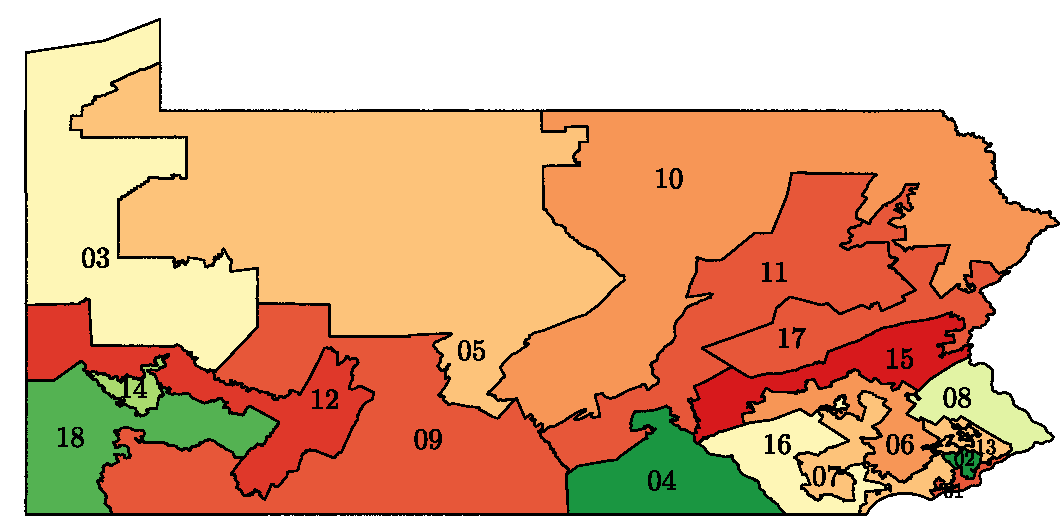
\includegraphics[width=0.48\textwidth]{map-moment_pop.pdf} \\ Moment of Population}
      \parbox{0.49\textwidth}{\centering \parbox{0.4\textwidth}{\caption{Compactness of Pennsylvania districts as computed by various metrics.  Green is the most compact, and red is the least.\label{f:compactnessmaps}}}}
    \end{center}
  \end{figure}

  While these measures generally correlate with each other, they do measure somewhat different things.  Figure~\ref{f:compactnessmaps} shows the compactness of each district in Pennsylvania by each compactness metric.  In general, the same districts tend to do well and badly by a number of metrics: for instance districts 2 and 4 are fairly compact by any measure, and districts 7 and 12 are not compact by any metric.  However, each does worse on some metrics and better on others.  For instance, district 7 has very low area compared to its perimeter, and its convex hull is giant compared to the district.  However, it is only somewhat more dispersed from its center than a compact district would be, so on the moment of area and moment of population metrics it does less poorly.  The barbell-shaped district 12 does poorly by moment of area and moment of population, but its boundary is fairly simple, so on the area-perimeter metric it does less poorly.

    \subsection{Partisan Symmetry and Vote Efficiency}
 While geographic compactness is a widely-considered metric for compactness, others have focused on actual results for determining unacceptable redistricting plans.  Over the last few years, the courts have increasingly rejected a variety of rationales cited to claim illegal gerrymandering, including ``partisan intent'',  ``minority party entrenchment'', and ``lack of proportionality''.  However, in \textit{League of United Latin American Citizens (LULAC) v. Perry, Governor of Texas et al.}, (2006), the majority recognized that it would accept a lack of \textit{symmetry} as an acceptable argument for determining unconstitutional gerrymandering.

  A given plan has symmetry if ``similary-situated parties are treated equally'', thus expecting that an even split in votes across two parties would have an even split in seats. Furthermore, if a plaintiff challenging a redistricting plan can demonstrate partisan intent and asymmetry, it would be sufficient for the burden of proof to shift to the state.  Nevertheless, while acknowledging the viability of symmetry as a metric to determine a discriminatory impact on voters, the court failed to establish an accepted standard or test to determine illegal gerrymandering.  Existing measures at the time, as calculated by social scientists, used hypothetical models to predict how election outcomes would turn out, given certain shifts in the electorate and certain vote shares in a given election. The court rejected the notion of using hypothetical models for a standard of constitutionality. \cite{LULAC}

  With this in mind,  as an alternative to other existing metrics, two legal scholars recently proposed measuring \emph{vote efficiency} as a way to quantify partisan symmetry and partisan gerrymandering~\cite{stephanopoulos}.  Vote efficiency is a measure of how well a given vote applied towards improving political representation.  In the case that a voter's desired candidate wins, any vote beyond what is necessary to win (in the simple case, 50\% + 1 vote) is wasted.  In the case when a voter's desired candidate loses, all votes for the losing candidate are wasted. Redistricting plans seeking a partisan bias will lead to fewer wasted votes for the favored party, while increasing wasted votes for the disadvantaged party.

  Vote efficiency helps to overcome several of the deficiencies expressed by the Supreme Court in \emph{LULAC}.  First, by using actual election data, rather than hypothetical models, the Court can establish a definite model for determining partisan bias.  Furthermore, it will allow the court to establish a test threshold for considering when a plan becomes unconstitutional.  This measurement will be explained precisely in the Methods section.

\subsection{Redistricting Processes}
Another key aspect when discussing gerrymandering is the political processes involved in redistricting.  The Constitution provides states with the ability to create their own rules in how districts are drawn, with the provisions that states will ensure balanced district populations, and that districts are redrawn at least every 10 years~\cite{LULAC}.

Currently, there are five general types of processes, some of which overlap.  The first, and most common, is when redistricting is done by the \emph{legislature}.    The legislature proposes plans and seeks to pass a bill for approval.  Sometimes, this may require a supermajority, or may be veto-proof, but typically requires simple majority approval from both the upper and lower houses and from the governor.  The second is the \emph{advisory commission} model, where a group of people, usually appointed officials, gather together to make non-binding recommendations to the legislature.  The third is the \emph{backup commission}, where failure of the legislature to pass a new plan triggers the activation of a predetermined committee to create an alternative.  The fourth is a \emph{political commission}, where elected officials often serve as members of a redistricting commission.  This is the sole legislative process for districting in New Jersey and Hawaii.  Last, \emph{independent commissions} are appointed groups of unelected officials independent of the legislature, who have full authority for developing new redistricting plans and require bipartisan or non-partisan composition.  This is the sole legislative process for districting in Arizona, Idaho, California, and Washington at the congressional level~\cite{Levitt}.

In addition to the overlap of legislature control and advisory or backup commissions, there are also some differences between the district drawing process for state legislatures and congressional districts.  For example, Pennsylvania's congressional districts are drawn by the state legislature whereas state legislative districts are drawn by a bipartisan political commission.  Furthermore, many states have different requirements for the composition of commissions, such as some states requiring bipartisan composition, with other states allowing elected officials to serve ex-officio.  Such distinctions create interesting results, as we will see in the Analysis section.

\subsection{Related Research}

In addition to proposing metrics for compactness and gerrymandering, a number of other authors have considered related approaches to measuring or understanding gerrymandering.  Several have investigated the question of the relationship between compactness and gerrymandering in hypothetical maps.  Chen and Rodden~\cite{chenrodden} drew random districts, using two different algorithms that attempted to draw compact and noncompact districts; they found that there was a general Republican bias due to political geography, and that this bias was slightly stronger when using the compact algorithm.  Altman~\cite{altman} drew different types of districts on hypothetical maps, and investigated the relationship between compactness, partisan bias, and other metrics.

Several authors have also looked at related questions on actual congressional maps.  Stephanopoulos~\cite{stephanopoulos2} investigated the effects of consequentialist legal requirements, such as requirements of partisan symmetry, and found that they were generally ineffective, and did consider compactness in passing, although it was not the focus of the work.  Fryer and Holden~\cite{fryer} compared ``maximally compact'' districts to the actual districts, and found them to exhibit less partisan bias.  However, to our knowledge, none have compared compactness and partisan bias on actual legislative or congressional districts.

  \section{Model}
  In this paper, we will conduct an analysis on the correlation between different measures of compactness and political bias, as a method for determining the overall asymmetry of a given political area.  Furthermore, we will examine the political processes involved in drawing those areas and compare the processes with the levels of gerrymandering exhibited.

  We expect to see the following in our results:
  \begin{itemize}
  \item Compactness and political bias/efficiency will correlate well, with population metrics and dispersion from center metrics performing more strongly than simple area and perimeter metrics
  \item Independent and bi-partisan commissions will outperform partisan legislative and advisory processes in producing less-gerrymandered districting plans.
  \end{itemize}

  We predict these outcomes on the following basis: non-compact districts are oftentimes designed in such a way that extensive work to include wide swaths of voters will lead to districts where people are spread out over a wide area or in a few very dense spaces.  Furthermore, these districts are designed to create partisan bias, not partisan fairness, and thus will correlate with the voter efficiency.  Also, we expect to find that partisan legislative process will more likely produce gerrymandered districts, as the lack the political checks and balances than an independent or bi-partisan political body would ensure.  While we do not expect all partisan legislative processes to have gerrymandered districts, we still expect that all gerrymandered districts will be created by partisan legislative processes.

  \section{Methods}

  \subsection{Computing Compactness}

  We used a number of the metrics discussed in Section~\ref{s:background} to measure the compactness of districts.  To compute them, we used the geographic data from the U.S.~Census's TIGER/Line database~\cite{censustiger} on the shapes of congressional districts and census blocks, and where applicable, population data from the 2010~Census~\cite{census2010}.

  The simplest metric we computed was $4\pi A/P^2$.  The only complication to computing this metrics was the handling of coastlines, for which the district boundary is generally drawn a few miles offshore.  Rather than try to resolve this issue by clipping the district to the coastline, and therefore potentially increasing the perimeter of the district due to the complexity of the coastline, we simply computed the perimeter and area as drawn; we think the error introduced this way is likely smaller than that introduced by attempting to correct for it.  We computed the moment of area in a similar way.

  Another purely geometric computation that we ran was the ratio of district area to area inside the convex hull of the district. For non-contiguous districts, which generally include islands, we simply computed one convex hull encompassing the entire district rather than trying to handle different sections separately. This results in some situations where a district is penalized for having a large area of water outside the district boundary. However, the alternative would fail to catch cases where a populated island is assigned to a district in an unreasonable way. Since both options have their drawbacks, we chose the one that simplified computation.

  The population moment of area was also simple to compute, since the TIGER/Line data approximates each district as a polygon.  Again, we ignored the issue of clipping to the coastline to avoid introducing more error.  Using census block population data, we also computed the population moment of inertia of each district.  We used the method described in Section~\ref{s:background} to deal with the limited granularity of the population data.

  The ratio of district population to population inside the convex hull of the district introduced another issue: determining population inside an arbitrary area. The available population data was by census block, so we had to compute which census blocks are inside each convex hull. We chose to count a census block as being ``inside'' the convex hull if the interior of the census block and the interior of the convex hull overlap. We ignored census blocks outside of the state that the district is in, even if those blocks might be inside the convex hull, since they are irrelevant for redistricting purposes and it is ideal to avoid penalizing states which are themselves not compact.

  With the non-population-based metrics especially, Alaska and Hawaii present particular difficulties, since they include a number of widely dispersed islands.  However, Alaska has only one representative, and Hawaii only two, so since our analysis focused on states with at least three districts, we did not attempt to resolve these issues.

  \subsection {Computing Voter Efficiency}
  We calculate voter efficiency using data from a variety of sources.  The US Census Data, along with the Harvard Election Data Archive~\cite{heda} presents a great resource for Federal Election results.  State-by-state elections are best sourced from the respective state agencies that govern the election, such as the Secretary of State's office or Board of Elections.  To calculate voter efficiency, we first go back to the definition of wasted votes.  This measure of voter efficiency will only analyze two-party, single-winner elections.  Thus, for a given party $p$, their opposing party $o$ and a given district $i$, the number of wasted votes  if party $p$ wins ($V_{p} > V_{o}$)  is given by
    \[ V_{wpi} = V_{pi} - \frac{V_{pi}+V_{oi}}{2}\]
  as all votes beyond 50\% are wasted. Otherwise, if party $p$ loses the district, then
    \[V_{wpi} = V_{pi}\]
  as all votes that do not go towards electing a candidate are wasted.

    While this calculates the wasted votes for an individual district, vote efficiency is calculated at the aggregate state level.  The vote efficiency $V_{Ep}$ for party $p$ is then calculated as follows:
     \[V_{Ep} = \frac{\sum_{i=1}^{n}\left(V_{wpi}-V_{woi}\right)}{\sum_{i=1}^{n}\left(V_{pi}+V_{oi}\right)}\]

     Stephanopoulos and McGhee also propose that $V_{pi}+V_{oi}$ remains constant, as the size of any district in a given state cannot vary significantly, thus requiring equality.  Under this assumption, where the total votes in any given district are constant at $V_{t} = V_{pi}+V_{oi}$, and party $p$ wins $m$ of $n$ seats, the above equation simplifies to:
     \[V_{Ep} = \left(\frac{m}{n}-0.5\right) - 2*\left(\frac{\sum^{n}V_{pi}}{\sum^n{V_t}}-0.5\right)\]

  The first term, $\left(\frac{m}{n}-0.5\right)$ represents the ``seat share'' or the proportion of seats that were won by party $p$ in excess (or deficient) of half the seats.  The second term represents the ``vote share'' or the proportion of the vote that was won by party $p$ in excess of half. The 0.5 adjustment terms are there so that a positive $V_{Ep}$ indicates that the given party has an advantage due to partisan gerrymandering and a disadvantage with a negative $V_{Ep}$.  Furthermore, it represents the proportion of seats lost due to this disadvantage.

  Overall, the voter share/seat share metric is much easier to calculate, as nothing needs to be known about the individual districts, but rather only the totals of the overall election.  However, as we will expose in the analysis and discussion sections, the assumption that all districts have the same total votes does not hold well due to turnout variance and creates issues when analyzing the data.


  \section{Analysis}

  \subsection{Compactness and Efficiency Gap}

  In order to determine the relationship between compactness and partisan bias in district drawing, we used the data we computed for congressional districts to run regressions.  We regressed both the seat share and wasted votes computations of efficiency gap, both as a percentage of the legislature and as a raw number of seats on each measure of compactness separately.  Since little gerrymandering is possible in states with only one or two districts, we excluded those states; we additionally ran each regression on those states that have at least ten districts, to see the effect on those larger states where more gerrymandering is possible.

  The regression coefficients are shown in Tables~\ref{t:efficiency3}~and~\ref{t:efficiency10}, and the raw scatterplots are shown in Figures~\ref{f:compactnessplots}~and~\ref{f:effgapplots}.  All but one coefficient was negative, suggesting that districts which are less compact tend to be more gerrymandered.  In the twenty regressions on the large states, 14 of the coefficients were statistically significant at the $p<.05$ level.  The results were much weaker when including the smaller states, presumably because smaller states have less gerrymandering, and therefore tend only to add noise to the data.  In the latter regression, only a few of the results were statistically significant, and in general they were stronger when considering the efficiency gap as an absolute number of seats, presumably for the same reason.

  Of the efficiency gap computations, the seat share computation appeared to actually have a stronger relationship to compactness, in spite of being a simplified metric.  However, due to the small sample size and the fact that the two metrics produce similar results in many states, this may not be a meaningful difference.  Of the compactness metrics, moment of area performed the best; convex hull area and moment of population also did well.  The area-perimeter metric was ineffective; it did correlate with the seat share, but less strongly, and there were several states with low district compactness with little partisan bias.  The convex hull population metric also did less well than the others.

  \begin{table}
    \begin{center}
      \begin{tabular}{lrrrr}\toprule
        \multirow{2}{*}{Metric} & \multicolumn{2}{c}{Efficiency gap (seats)} & \multicolumn{2}{c}{Efficiency gap (\%)} \\
               & \multicolumn{1}{c}{Seat share} & \multicolumn{1}{c}{Wasted votes} & \multicolumn{1}{c}{Seat share} & \multicolumn{1}{c}{Wasted votes} \\\midrule
        \multirow{2}{*}{Area vs.~Perimeter} & -3.24 & -3.26 & -18.1 & -6.6 \\
        & (1.81) & (2.04) & (14.4) & (14.7) \\\midrule
        \multirow{2}{*}{Convex Hull Area} & -3.80 & -3.73 & -13.4 & 1.0 \\
        & (2.00) & (2.26) & (16.2) & (16.4) \\\midrule
        \multirow{2}{*}{Convex Hull Population} & -2.45 & -2.24 & -16.4 & -10.4 \\
        & (1.76) & (1.99) & (13.8) & (14.0) \\\midrule
        \multirow{2}{*}{Moment of Area} & -5.67* & -5.63 & -19.1 & -6.8 \\
        & (2.52) & (2.85) & (20.6) & (21.0) \\\midrule
        \multirow{2}{*}{Moment of Population} & -0.69* & -0.71* & -3.3 & -1.6 \\
        & (0.29) & (0.33) & (2.4) & (2.4) \\\bottomrule
      \end{tabular}
      \caption{Regression coefficients for efficiency gap regressed over each compactness metric separately on all states with at least three districts.  * denotes $p<.05$ (two-tailed test); standard errors in parentheses.\label{t:efficiency3}}
    \end{center}
  \end{table}

  \begin{table}
    \begin{center}
      \begin{tabular}{lrrrr}\toprule
        Metric & \multicolumn{2}{c}{Efficiency gap (seats)} & \multicolumn{2}{c}{Efficiency gap (\%)} \\
               & \multicolumn{1}{c}{Seat share} & \multicolumn{1}{c}{Wasted votes} & \multicolumn{1}{c}{Seat share} & \multicolumn{1}{c}{Wasted votes} \\\midrule
        \multirow{2}{*}{Area vs.~Perimeter} & -7.92 & -9.91 & -76.2* & -84.3* \\
        & (5.10) & (6.03) & (34.4) & (36.4) \\\midrule
        \multirow{2}{*}{Convex Hull Area} & -13.50* & -16.12* & -114.2* & -126.2* \\
        & (5.77) & (6.90) & (38.8) & (40.7) \\\midrule
        \multirow{2}{*}{Convex Hull Population} & -9.49* & -9.75 & -72.0* & -70.6 \\
        & (4.24) & (5.36) & (30.7) & (34.3) \\\midrule
        \multirow{2}{*}{Moment of Area} & -15.99** & -16.55* & -125.8** & -128.9** \\
        & (4.22) & (5.81) & (27.8) & (32.3) \\\midrule
        \multirow{2}{*}{Moment of Population} & -2.91 & -3.31 & -26.0* & -26.8* \\
        & (1.38) & (1.68) & (9.1) & (10.1) \\\bottomrule
      \end{tabular}
      \caption{Regression coefficients for efficiency gap regressed over each compactness metric separately on all states with at least ten districts.  * denotes $p<.05$, ** denotes $p<.01$ (two-tailed test); standard errors in parentheses.\label{t:efficiency10}}
    \end{center}
  \end{table}

  \begin{figure}
    \begin{center}
      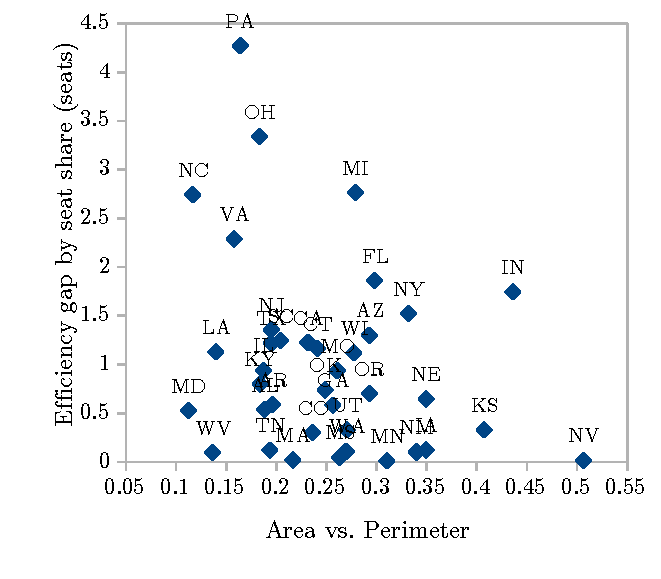
\includegraphics[width=0.49\textwidth]{sss-area_per.pdf}
      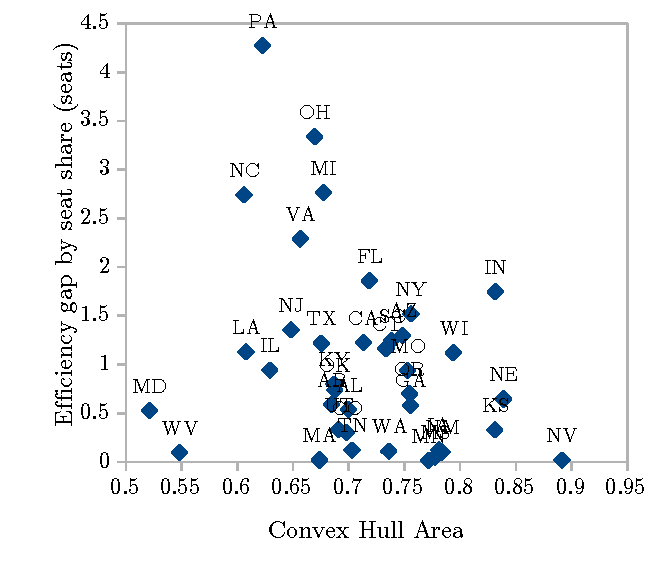
\includegraphics[width=0.49\textwidth]{sss-convex_hull.pdf}

      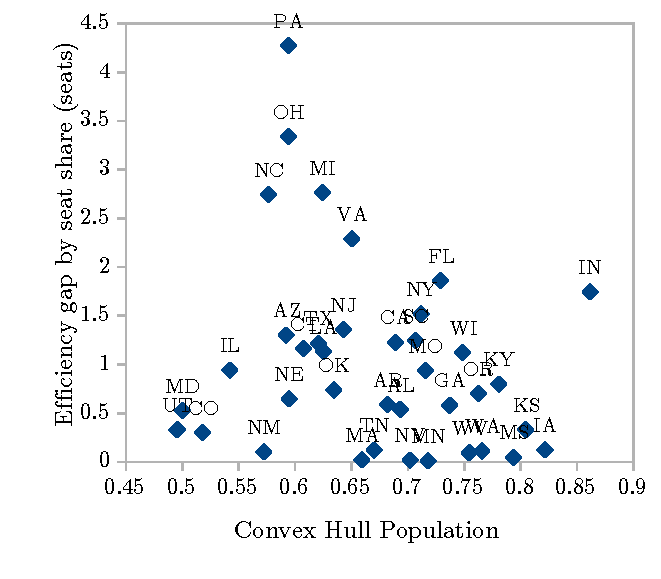
\includegraphics[width=0.49\textwidth]{sss-convex_hull_pop.pdf}
      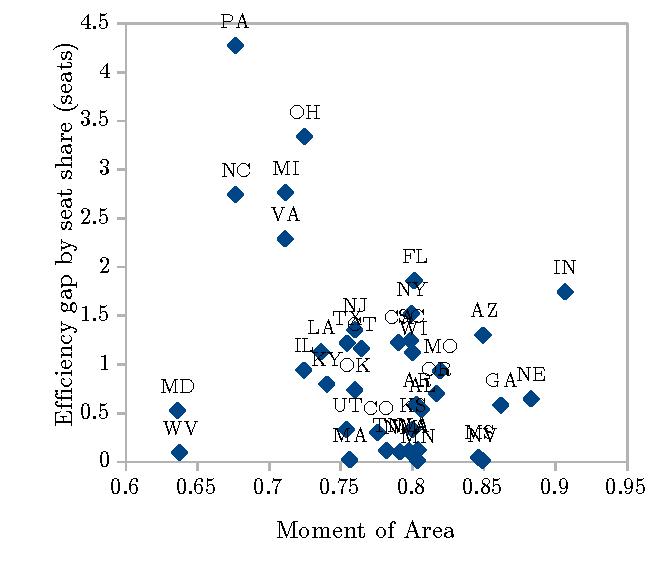
\includegraphics[width=0.49\textwidth]{sss-moment_area.pdf}

      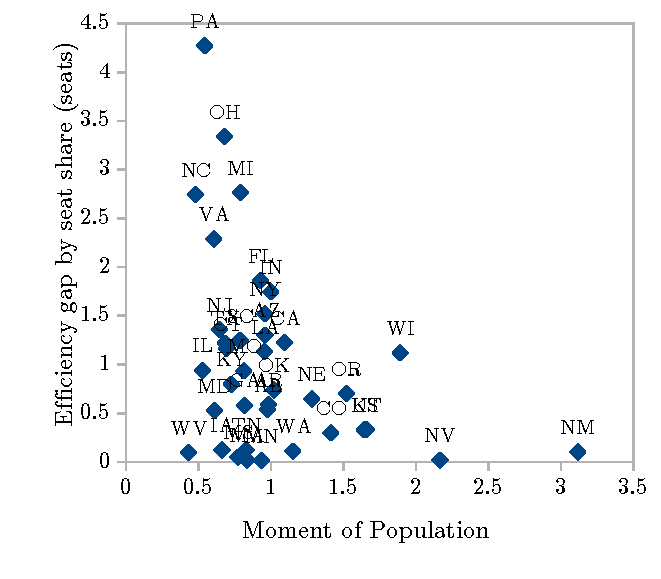
\includegraphics[width=0.49\textwidth]{sss-moment_pop.pdf}
      \parbox[b][2.8in][c]{0.49\textwidth}{\centering \parbox{0.4\textwidth}{\caption{Plots of efficiency gap (as computed by seat share, in seats) against each compactness metric.\label{f:compactnessplots}}}}
    \end{center}
  \end{figure}

  \begin{figure}
    \begin{center}
      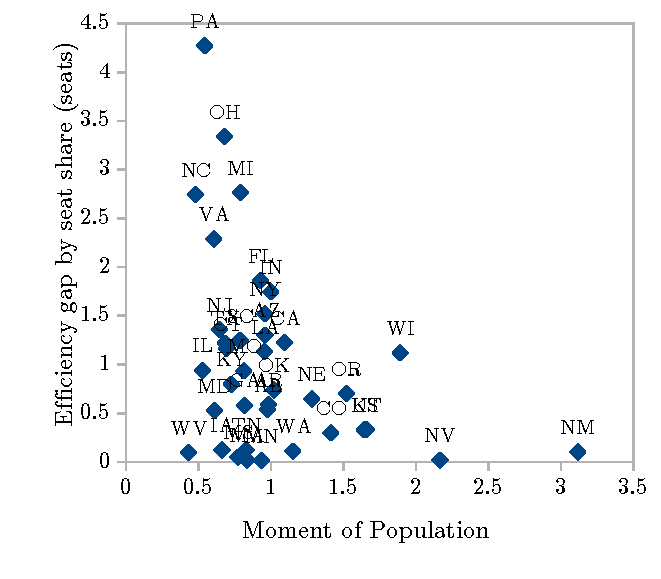
\includegraphics[width=0.49\textwidth]{sss-moment_pop.pdf}
      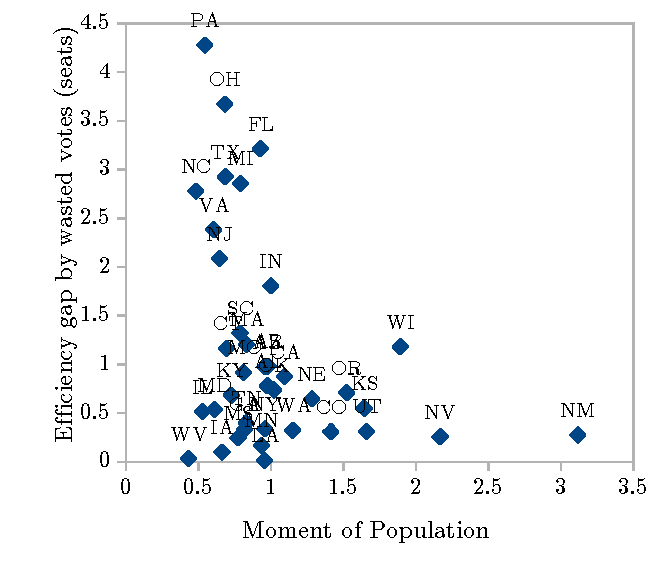
\includegraphics[width=0.49\textwidth]{wvs-moment_pop.pdf}

      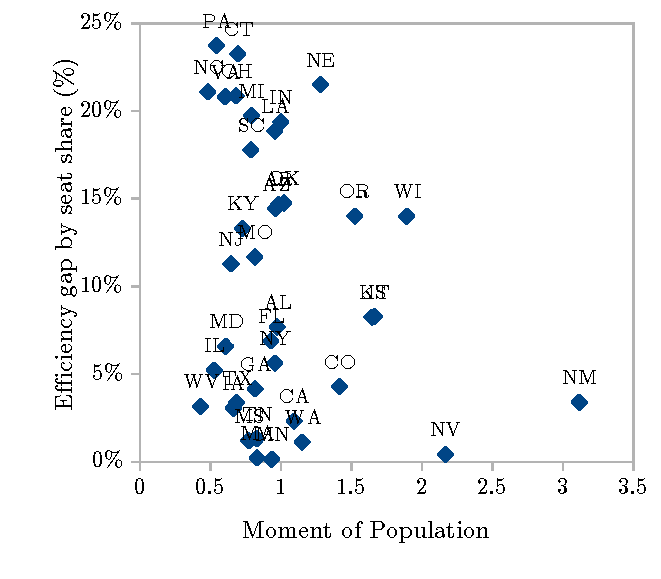
\includegraphics[width=0.49\textwidth]{ssp-moment_pop.pdf}
      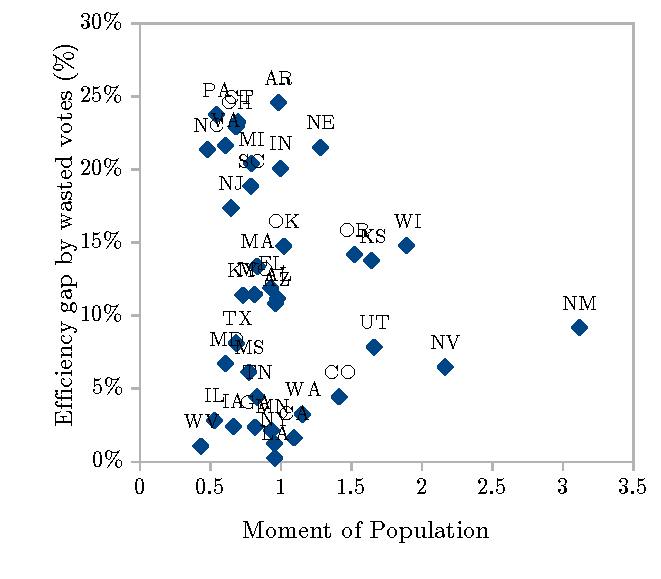
\includegraphics[width=0.49\textwidth]{wvp-moment_pop.pdf}

      \caption{Plots of each efficiency gap computation against compactness as measured by moment of population.\label{f:effgapplots}}
    \end{center}
  \end{figure}

  We also analyzed some of the state legislatures.  Unfortunately, the data for these races is not as easily accessible, so we had to record it manually from the websites of various Secretaries of State and Boards of Elections~\cite{heda,florida,georgia,illinois,newyork,washington}, and we were only able to collect and analyze the data for a few of the largest states' lower houses.  Because of the limited amount of data, none of the regression coefficients were statistically significant, although they all had the right sign.  Scatterplots for two of the stronger results are shown in Figure~\ref{f:stateplots}.

  \begin{figure}
    \begin{center}
      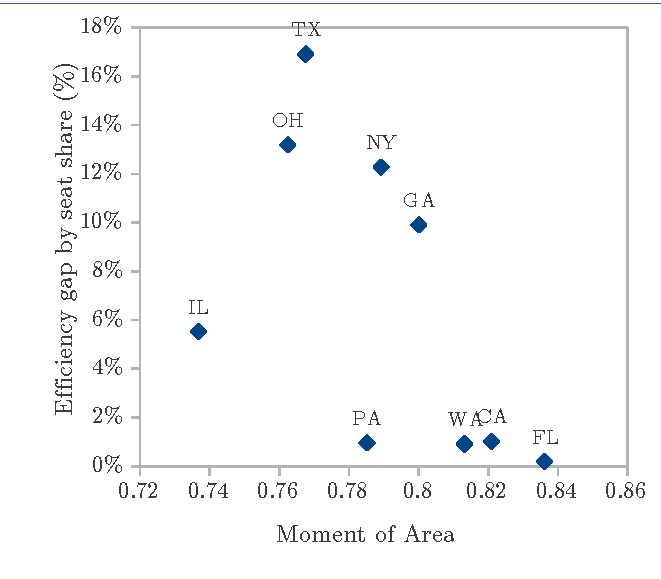
\includegraphics[width=0.49\textwidth]{sldl-ssp-moment_area.pdf}
      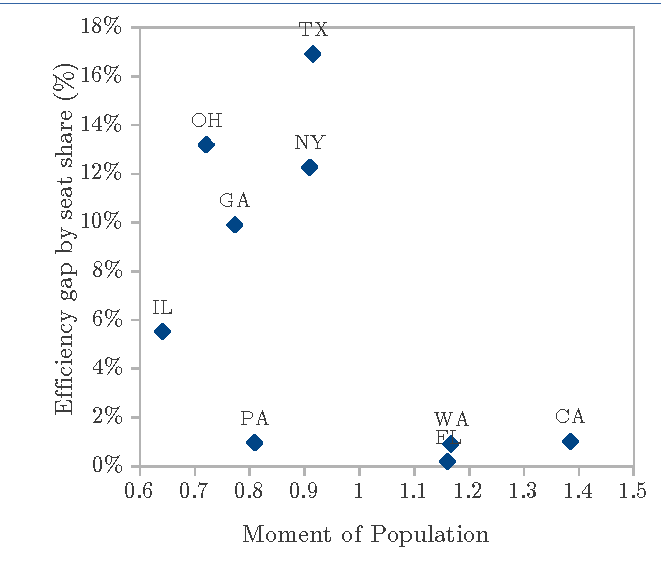
\includegraphics[width=0.49\textwidth]{sldl-ssp-moment_pop.pdf}

      \caption{Plots of efficiency gap as measured by seat share, as a percentage of the legislature, against moment of area and moment of population.\label{f:stateplots}}
    \end{center}
  \end{figure}


 \subsection{Redistricting Processes}
Taking in the states with at least 10 congressional districts, using both compactness and vote efficiency as a metric for measuring gerrymandering, we also find that legislative processes for redistricting produce more gerrymandered districts. The top half of states by each metric (Pennsylvania, Ohio, North Carolina, Michigan, and Virginia for both metrics, Texas for vote efficiency, and Illinois for compactness) all use legislative redistricting processes.  Likewise, three of the five states (California, Washington and New Jersey) in the bottom half of gerrymandering as measured by both metrics employ independent redistricting commissions or equally partisan political commissions.
Looking into this process further, we see this disparity even further in some of the most prominent of gerrymandered states -- Pennsylvania.  In Pennsylvania, the state legislature's Congressional plan produced an efficiency gap of nearly 24\%, or 4.27 seats.  However, the state house districts produced a seat gap of less than one -- out of over 200 seats.  This state house plan was drawn by an equally partisan political commission with representatives selected evenly by each party, thus forcing the state house districts to be drawn in a fair manner.  On the other hand, the Republican state legislature then subsequently forced through the plan that created the 4-seat bias, including a 26-24 vote in the state senate, with all Democrats and a few Republicans voting against the clearly gerrymandered plan.  The nature of such a biased legislative process clearly can lead to inequality in the system.

With the aforementioned data considered, several states do not observe the same trend.  For example, Georgia ranks highly on compactness and partisan bias metrics, and does not appear to be very gerrymandered.  However, it has a legislative process to draw congressional districts, and has a fairly partisan Republican state legislature.  While we would expect to see a more gerrymandered district, it appears as though that is not the case.  One possible explanation for this phenomenon is that several Democratic Congressmen from Georgia, such as John Barrow, are often more conservative than their counterparts from other states in Congress.  It was not until after 2000 that the state shifted to Republican dominance, and even then, some Democrats have managed to retain their seats.  While states such as Georgia appear to have a fair system, opening redistricting to a solely legislative process opens the opportunity for abuse.

  \section{Discussion}
  \subsection{Usefulness of Different Metrics}
  \subsubsection{Compactness Metrics}
  As measures for gerrymandering, none of the measures of compactness alone is a perfect measure.  In each case, there were some states that scored poorly on a compactness metric, but for which there was no evidence of partisan gerrymandering.  It is possible that in these cases there was a bipartisan gerrymander, or a gerrymander which did not happen to cause many wasted votes in the election we considered; our data are insufficient to decide.  In addition, our data cannot show a causal relationship.  In particular, while gerrymandering may cause noncompact districts, it could also be the case that states which tend to draw heavily gerrymandered districts also tend to draw noncompact districts.  However, the presence of noncompact districts does seem to generally indicate that there may be gerrymandering, and conversely states with compact districts tended to have low partisan bias.

  The individual metrics also did not perform equally well.  The area-perimeter metric did not perform particularly well, as might be expected from its simplicity: the relationship was in the right direction, but was comparatively weak.  The moment of area and moment of population preformed quite well.  Oddly, moment of area in fact did better than moment of population; we conjecture that this is due to the difficulty of properly normalizing this metric for districts of different sizes and populations.

  Metrics that use the convex hull of a district are based on the observation that problematic districts are likely to have a section ``cut out'', jut out into a neighboring district, or stretch out in a long, narrow, curved line. Like the perimeter metric, they disadvantage districts with jagged boundaries, although less heavily. The purely geometric version, like other compactness metrics, penalizes states that are non-compact. It particularly affects states that are on a coast and have islands, because a large offshore area gets counted in the convex hull. For example, California's 14th district gets an especially bad score because it combines a small, densely populated area with a group of islands several miles offshore. However, the population-based version does not have these issues. In cases where a state has complex boundaries with other states, the population outside of the state can simply be ignored. In cases where a state has islands, the offshore area has no population so it has no effect. Despite these advantages, the population-based version still performed worse overall. Many states have suburban districts that wrap around a city, and even when these are drawn in a fairly reasonable way, the city still tends to be included in the convex hull, and the district gets heavily penalized, especially in the population-based version.

  \subsubsection{Voter Efficiency}
  As we have seen, voter efficiency works well as a measure for illegal gerrymandering, especially in concert with a good measure of compactness.  However, it does fall short in some situations.  For example, it does a poor job of measuring gerrymanders designed to protect incumbents.  In such a case, each party might waste a comparable number of votes, designed to protect the legislators still in office.  The voter efficiency gap would be low, yet districts would be predictable in outcome, protecting the incumbent.

  Similarly, races that are not contested can produce an extreme number of wasted votes for the winning party, with half of the total votes in that district being considered wasted.  While this may be indicative of partisan gerrymandering, it may also be reflective of a legislature people aren't as interested in.

  Third, the voter efficiency gap is an extremely volatile measure.  Especially at the state house level, where representatives will be elected by only a few tens of thousands of voters, changes in the composition of the electorate can dramatically alter the quantities of votes wasted.  A seat flip in a close election can dramatically alter the amount of wasted votes for each party, essentially swapping the number of wasted votes.  In today's electorate, this could easily happen, in particular with the growing minority population.

  Finally, we find that Stephanopolous and McGhee's simplification of wasted votes into seat share and vote shares simply does not work.  For states where districts are not well-contested, voter efficiency measures can dramatically change from favoring one party slightly to favoring the other party significantly.  In one case, we saw Texas go from approximately one seat pro-democratic, to over two seats pro-republican.  Thus, the wasted votes approach, as the more general case, is much better to use for consistency and accuracy reasons.
  
  \subsection{Standards for Gerrymandering}

  Taken together, efficiency gap and compactness can give a very strong indication of gerrymandering.  If a state has noncompact districts, this suggests that the districts may have been drawn unfairly; partisan bias can confirm the particular type of advantage they give.  Conversely, high partisan bias might be justifiable if a districting plan is compact, on the basis that the political geography naturally benefits one side, as Chen and Rodden suggest.~\cite{chenrodden}  In addition, this relationship gives a framework for evaluating compactness metrics and other metrics of gerrymandering: if a metric tends to correlate with the other existing metrics of gerrymandering, it can be used as an additional indicator.

  Based on the data we have gathered, we propose an extension to the test of Stephanopoulos and McGhee~\cite{stephanopoulos}.  At a congressional level, we propose that districting plans for states with at least 3 districts be overturned if they have an efficiency gap of greater than 20\% or two seats, and also register poorly on at least one compactness metric: below $\frac23$ in the convex hull area metric, below $\frac34$ in the moment of area metric, or below $\frac23$ in the moment of population metric.  This weakens the standard 

  We believe that this accurately captures the most egregious of gerrymandering, as for states with at least 3 congressional districts, a 20\% threshold limit or 2 seat gap creates a balance to test for gerrymandering in both small and large states.  For small states, this could mean a seat distribution changing from 3-0 to 2-1, which is small on the grand scale, but possibly offers better representation within that state. Likewise, it can catch large states, who can have a strong influence on the overall makeup of Congress.  Based on our data, it would invalidate districting plans in Michigan, New Jersey, North Carolina, Ohio, Pennsylvania, and Virginia on the basis that they have a gap larger than two seats and the requisite compactness.  A few other states, such as Connecticut and Nebraska, meet the partisan bias standard, but not the compactness standard, so they would not be invalidated.  Providing this criteria will allow the courts to effectively decide on gerrymandering cases.

  We also propose that states revise their policy on allowing state legislatures to draw lines independently.  Nonpartisan and balanced partisan processes create fair, consensus plans, as they will require agreements that prevent the parties from simply passing a partisan bill designed to reduce the prevalence of partisan gerrymandering.

  \section{Conclusion}
  Partisan gerrymandering damages the fundamental nature of our representative democracy.  It produces unfair advantages that prevent citizens from being represented fairly.  Real redistricting is too complex for a single simple metric to be able to quantify all types of gerrymandering, but by combining multiple metrics, it is possible to catch a number of different types of gerrymanders in a specific and quantifiable way.  Using quantifiable metrics of partisan gerrymandering, we hope to create a standard that can delineate results that are blatantly biased, regardless of any ability to discover the intent of those who created the plans.


  \singlespacing{}

  \printbibliography{}

\end{document}
